\chapter[short]{一般滤波器的程序设计}

对信号的时间演化过程进行估计十分常见。一般来说,信号可以分为周期信号(有限带宽信号、确定性信号)与随机信号(无限带宽信号、
随机信号)。对于确定信号滤波侧重于对信号不同频谱分量的取舍,例如低通滤波器保留信号的低频分量,丢弃信号的高频分量。因此这种
滤波器也称作频率成型滤波器\cite{oppenheim1997signals}。对于随机信号,滤波侧重其功率谱不同分量的取舍,在时间域对应的操作
就是对自相关函数的修改。随机信号滤波本质是对其时间统计特征和概率特征的成型。因此,滤波器的设计准则也将基于相关统计特征,
这和确定性信号滤波有显著的不同。但这两种滤波方式并非对立,对随机过程的滤波操作都可以归纳到统一数学框架中,视作在频率与
时域上修改了统计特性。根据使用滤波器目的不同与信号本身特性,不同滤波方法只是各自侧重比例不同而已。

假设要对某随机过程 $t=n$ 时刻的值进行估计,根据可用数据因果性,有三种主要的任务形式\cite{theodoridis2020machine}:
\begin{itemize}
    \item  滤波,在时刻 $n$ 的估计是基于所有先前的接受(测量)输入信息,\emph{直到并包括}当前时刻 $n$。
    \item  平滑,首先收集时间区间 $[0,N]$ 内的数据,使用区间 $[0,N]$ 中\emph{所有}可用信息,得到每个时刻 $t\le N$ 的估计。
    \item  预测,基于直到包括时刻 $n$ 的信息,得到 $n+ \tau,\tau\ge 0$ 的估计。
\end{itemize}

举一个时变随机过程例子:时刻 $n$ 的输出变量是 $y_n$,其值取决于相应的输入向量 $x_n$ 包含的观测值。在滤波中,
后者只能包括时刻 $n,n-1,\dots ,0$。索引集中这种限制表明了因果关系。相反,在平滑过程中,除了过去时刻的数据,还能使用
未来时刻的信息,即 $\dots ,n+2,n+1,n,n-1,\dots $。

三种任务形式本质上同源,只是根据时间因果性进行区分。因此很多算法稍作改变就能互通:如 Savizkg-Golay 平滑算法被称作
Savizkg-Golay 滤波器;均值滤波器的与滑动平均有同样的数学表达。在本章除有特殊情况,以滤波算法代替作为说明。

\section{线性滤波}

线性滤波指滤波器输出是输入\emph{线性叠加}的滤波器。由于它的频域特性是固定的,因此最适用于处理周期信号,也因为结构简单,
除一般软件实现外,还广泛存在于硬件电子电路与机械物理结构中。

\subsection{基本特性}
数字滤波器的数学模型如下:设输入信号为 $x(n)$,输出信号为 $y(n)$,滤波过程可用以下差分方程来表示\cite{scipy_docs_filtering}:
\begin{equation}
    \label{flt_time_domain}
    a_0y_{n}=\sum_{i=0}^{N} b_{i} x_{n-i}-\sum_{j=1}^{M-1} a_{j} y_{n-j}
\end{equation}

其对应的传递函数\footnote[1]{请注意识别系数中的项数与 $a,b$ 代表的含义,它们往往在不同文档与程序中不同甚至相反。}为:
\begin{equation}
    H(z)=\frac{\sum\limits_{i=0}^{N} b_iz^{-i}}{1+\sum\limits_{i=1}^{M-1} a_iz^{-i}}
\end{equation}

它对单位冲激函数的响应为:
\begin{equation}
    \begin{split}
        \label{h_resp}
        h_n=z^{-1}(H(z))\\
        y_n=\sum_{i=-\infty}^{\infty} h_ix_{n-i}
    \end{split}
\end{equation}

设计线性滤波器就是找到合适的 $h(n)$,使输出信号满足使用需求。通过观察式 \eqref{h_resp} 给出的时域输出,可以讨论一些数字滤波器中
共通的基本特性与常见概念。首先是递归特性(Recursive Filter):

当 $a_0=1$,其余 $a_k$ 均为零时,称滤波器是非递归的,又称\emph{有限冲激响应}(Finite Impulse Response, FIR)滤波器;该类型
滤波器也称为移动平均(MA)滤波器。当 $a_0 = 1$,其余 $a_k$ 不全为零时,称滤波器为递归的,又称\emph{无限冲激响应}(Infinite
Impulse Response, IIR)滤波器;该类型滤波器根据是否满足 $b_0 = 1$ 且 $b_k = 0$,又分为自回归(AR)滤波器与自回归
移动平均(ARMA)滤波器\cite{hamilton2020time}。值得注意的是:虽然一般将递归与 IIR 滤波器对应,非递归与 FIR 滤波器对应,但它们之
间关系不是严格等同的,递归同样适用于 FIR 滤波器实现,非递归也可实现 IIR 滤波器。
\begin{tcolorbox}
    \textrm{根据随机过程区分类型:}
    \begin{align*}
        y_{n} & =\sum_{i=0}^{N} b_{i} x_{n}\qquad                                & \textrm{MA,移动平均过程}      \\
        y_{n} & =x_{n}-\sum_{j=1}^{M-1} a_{j} y_{n-j}\qquad                      & \textrm{AR,自回归过程}       \\
        y_{n} & =\sum_{i=0}^{N} b_{i} x_{n}-\sum_{j=1}^{M-1} a_{j} y_{n-j}\qquad & \textrm{ARMA,自回归移动平均过程}
    \end{align*}
\end{tcolorbox}


其次是因果性(Causal Filter):如果对于 $n< 0$ 时,脉冲响应系数 $h(n)$ 不为零,则说明系统某时刻输出与未来输入相关,不具有因果性;
否则称滤波器是\emph{因果系统}。当冲激响应系数满足以下条件时,称系统是因果且稳定的:
\begin{equation}
    \begin{cases}
        h(n)=0, n\le 0 \\
        \sum_{n=0}^{\infty} \vert h(n) \vert \le C
    \end{cases}
\end{equation}

这些概念都容易从直观上解释:例如对于某滤波器,等式右边项 $y$ 相关系数全零时,系统只与过去时刻输入有关,因此具有有限项、因果性、
绝对稳定性;当右边项 $y$ 相关系数不为全为零,相应系数的引入相当于对原系统增加反馈环节,等同于追加入无穷多项输入,改变了原有
因果与稳定性。

\subsection{FIR 滤波器}

在线性滤波器中,FIR 滤波器又是最简单的滤波器:它等价于开环系统,拥有绝对稳定性,并且容易设计出\emph{线性相位}\cite{enwiki:1140890375}系统。
这使得设计良好的 FIR 滤波器对周期信号的行为是十分明确易知的。
\subsubsection{相幅特性}
式 \eqref{h_resp} 给出了滤波器的频幅响应与相位偏移。考虑到任务因果性,滤波器对于负时间的响应为零。对于输入长度为 $N$,采样周期
为 $T$ 的信号序列,滤波器输出响应与信号序列中点 $M$ 有如下的关系:
\begin{itemize}
    \item \uppercase\expandafter{\romannumeral1} 型\footnote[1]{这种分类在使用滤波器程序设计工具,如 fir1 时常见。}:信号序列长度是奇数
          $N=2M+1$,存在确实中点 $M$,且系数 $h[n]$ 围绕该中点偶对称分布:
          \begin{align*}
              \mathrm{H}(j \Omega) & =\sum_{n=-M}^{M} h[n] \cdot e^{-j \Omega T(n+M)}                                      \\
                                   & =e^{-j \Omega T M} \sum_{n=-M}^{M} h[n] \cdot e^{-j \Omega Tn}                        \\
                                   & =e^{-j \Omega T M}
              \left\{
              h[M]+\sum_{n=0}^{M-1} h[n] \cdot\left(e^{j \Omega T n}+e^{-j \Omega T n}\right)
              \right\}                                                                                                     \\
                                   & =e^{-j \Omega T M}\left\{h[M]+\sum_{n=0}^{M-1} h[n] \cdot 2 \cos (\Omega T n)\right\}
          \end{align*}
          表明该系统对频率 $\Omega$ 谐波会产生 $-\Omega TM$ 线性相位偏移,此斜率即\emph{群延迟}\cite{oppenheim1997signals}。
          FIR 滤波器有着线性相位偏移:即对任何频率谐波成分,有同样的群延迟,对应于整个系统输入延迟 $TM$ 时间。注意线性相位是由 $h(n)=h(2M-n)$
          保证的。
    \item \uppercase\expandafter{\romannumeral2} 型:任务信号序列长度是偶数 $N=2M$,存在虚拟中点 $M-\frac{1}{2}$,且系数 $h[n]$ 围绕该
          中点偶对称分布:
          \begin{align*}
              \mathrm{H}(j \Omega) & =\sum_{n=-M}^{M-1} h[n] \cdot e^{-j \Omega T(n+M)} \\
                                   & =\sum_{n=\frac{1}{2}}^{M-\frac{1}{2}}
              \left\{
              h[M-\frac{1}{2}-n] \cdot e^{-j \Omega T(M-\frac{1}{2}-n)}+
              h[M-\frac{1}{2}+n] \cdot e^{-j \Omega T(M-\frac{1}{2}+n)}
              \right\}                                                                  \\
                                   & =\sum_{n=0}^{M-1}
              \left\{
              h[M-n-1] \cdot e^{-j \Omega T(M-n-1)}+ h[M+n] \cdot e^{-j \Omega T(M+n)}
              \right\}                                                                  \\
                                   & =e^{-j \Omega T (M-\frac{1}{2})}
              \left\{
              \sum_{n=0}^{M-1} h[M+n] \cdot\left(e^{j \Omega T(n+\frac{1}{2})}+e^{-j \Omega T(n+\frac{1}{2})}\right)
              \right\}                                                                  \\
                                   & =e^{-j \Omega T (M-\frac{1}{2})}
              \left\{
              \sum_{n=0}^{M-1} h[M+n] \cdot 2 \cos \left[\Omega T (n+\frac{1}{2})\right]
              \right\}
          \end{align*}
          表明该系统对频率 $\Omega$ 谐波会产生 $-\Omega T(M-\frac{1}{2})$ 线性相位偏移,当 $\Omega=\pi$ 时,
          $\cos \left[\Omega T (n+\frac{1}{2})\right]=0$,故 $\mathrm{H}(j\Omega)=0$,即该类型滤波器
          不能用于$H(\pi)\ne 0$ 的滤波任务,此时线性相位特性与实现高通、带阻滤波器要求相矛盾。
    \item \uppercase\expandafter{\romannumeral3} 型:任务信号序列长度是奇数 $N=2M+1$,存在确实中点 $M$,且系数 $h[n]$ 围绕该中点奇对称分布:
          \begin{align*}
              \mathrm{H}(j \Omega) & =\sum_{n=-M}^{M} h[n] \cdot e^{-j \Omega T(n+M)}                                   \\
                                   & =e^{-j \Omega T M} \sum_{n=-M}^{M} h[n] \cdot e^{-j \Omega Tn}                     \\
                                   & =e^{-j \Omega T M}
              \left\{
              \sum_{n=0}^{M-1} h[n] \cdot\left(e^{j \Omega T n}-e^{-j \Omega T n}\right)
              \right\}                                                                                                  \\
                                   & =-je^{-j \Omega T M}\left\{\sum_{n=0}^{M-1} h[n] \cdot 2 \sin (\Omega T n)\right\}
          \end{align*}
          表明该系统对频率 $\Omega$ 谐波会产生 $-(\Omega+\frac{\pi}{2}) TM$ 线性相位偏移,由于在 $\Omega=\pi$ 处频幅响应为零,
          不能用于 $H(\pi)\ne 0, H(0)\ne 0$ 的滤波任务,可以实现带通滤波器。
    \item \uppercase\expandafter{\romannumeral4} 型:任务信号序列长度是偶数 $N=2M$,存在虚拟中点 $M-\frac{1}{2}$,且系数 $h[n]$ 围绕
          中点奇对称分布:
          \begin{align*}
              \mathrm{H}(j \Omega) & =\sum_{n=-M}^{M-1} h[n] \cdot e^{-j \Omega T(n+M)} \\
                                   & =\sum_{n=\frac{1}{2}}^{M-\frac{1}{2}}
              \left\{
              h[M-\frac{1}{2}-n] \cdot e^{-j \Omega T(M-\frac{1}{2}-n)}+
              h[M-\frac{1}{2}+n] \cdot e^{-j \Omega T(M-\frac{1}{2}+n)}
              \right\}                                                                  \\
                                   & =\sum_{n=0}^{M-1}
              \left\{
              h[M-n-1] \cdot e^{-j \Omega T(M-n-1)}+ h[M+n] \cdot e^{-j \Omega T(M+n)}
              \right\}                                                                  \\
                                   & =e^{-j \Omega T (M-\frac{1}{2})}
              \left\{
              \sum_{n=0}^{M-1} h[M+n] \cdot\left(e^{j \Omega T(n+\frac{1}{2})}-e^{-j \Omega T(n+\frac{1}{2})}\right)
              \right\}                                                                  \\
                                   & =-je^{-j \Omega T (M-\frac{1}{2})}
              \left\{
              \sum_{n=0}^{M-1} h[M+n] \cdot 2 \sin \left[\Omega T (n+\frac{1}{2})\right]
              \right\}
          \end{align*}
          表明该系统对频率 $\Omega$ 谐波会产生 $-\Omega T(M-\frac{1}{2})$ 线性相位偏移,并且当 $\Omega=0,2\pi$
          时频幅响应为零,不能实现低通、带阻滤波器。注意以上所有要求与分析只适用于因果线性相位 FIR 滤波器。FIR 滤波器不需要满足这些特性时,
          项数与系数、实现的滤波器类型之间没有关系。
\end{itemize}

\subsubsection{窗函数法}

FIR 滤波器的系数设计有多种方法。最常见的一种是首先根据滤波类型(低通/高通/带通/带阻)选择理想的频率响应,然后与频域上特定形状的函数
做卷积,达到频率选择成型的目的。该过程中使用的函数称作窗函数,这种方法称为窗函数法。
\begin{figure}[htbp]
    \centering\label{ideal_lp_g_resp}
    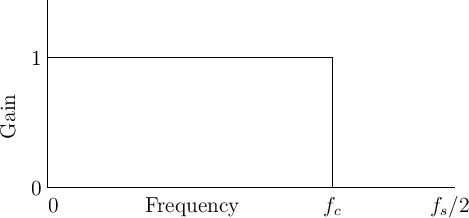
\includegraphics[width=0.5\textwidth]{ideal_lp_flt_am_G.png}
    \caption{理想低通滤波器幅值频幅响应}
\end{figure}

对于给定的 FIR 系统,其时域输出由输入频谱 $X(\Omega)$ 和滤波器频响 $H(\Omega)$ 乘积的逆离散傅里叶变换($\rm{DTFT^{-1}}$)给出:
\begin{equation}
    \label{fir_y_t}
    y(n)=\textrm{DTFT}^{-1}_n(H\cdot X)=\frac{1}{2\pi}\int_{-\pi}^{\pi}H(\Omega)X(\Omega)e^{j\Omega n}d\Omega
\end{equation}
其中 $\rm{DTFT}$ 定义为:
$$
    \textrm{DTFT}_{\Omega}(x)=\sum_{n\in \mathbb{Z}}x(n)e^{-j\Omega n}
$$
输出信号的频谱形状决定了式\eqref{fir_y_t}中冲激响应系数计算方式。以设计理想低通滤波器为例,其频谱应在频率从零到截至频率 $f_c$ 的通频带
内具有单位增益,在截止频率 $f_c$ 以上时,具有增益零(图\ref{ideal_lp_g_resp}):
\begin{equation*}
    H(\Omega)=\begin{cases} 1\quad(-\Omega_c\le\Omega\le \Omega_c)\\ 0\quad(else) \end{cases}
\end{equation*}
为找到满足该特性的响应系数,作逆离散傅里叶变换:
\begin{equation}
    h[n]=\frac{1}{2\pi}\int_{-\Omega_c}^{\Omega_c}{1\cdot e^{j\Omega n}d\Omega}
    % =\frac{1}{2\pi}[\frac{e^{j\Omega n}}{jn}]_{-\Omega_c}^{\Omega_c}
    =\frac{\sin(2\pi f_c n)}{n \pi}
    =\Omega_c \frac{\sin \left(n \Omega_{c}\right)}{\left(n \Omega_{c}\right)}
    =B \textrm{sinc}(Bn)
\end{equation}
其中 $\Omega_c=2\pi f_c$ 为角频率,$B = 2f_c$ 为通频带宽,$\textrm{sinc}$ 是\emph{辛格函数}。同理,可以得出理想高通、带通、带阻滤波
器的响应系数表达式:
\begin{table}[!h]
    \caption{理想滤波器频幅响应系数}
    \centering
    \begin{tabular}{ccc}
        \hline
        类型 & $h[n],n\ne0$                                    & $h[n],n=0$ \\ \hline
        低通 & $B\mathrm{sinc}(Bn)$                            & $B$        \\
        高通 & -$B\mathrm{sinc}(Bn)$                           & $1-B$      \\
        带通 & $B_2\mathrm{sinc}(B_2n)-B_1\mathrm{sinc}(B_1n)$ & $B_2-B_1$  \\
        带阻 & $B_2\mathrm{sinc}(B_2n)+B_1\mathrm{sinc}(B_1n)$ & $B_2+B_1$  \\ \hline
    \end{tabular}
\end{table}

由于理想滤波器输出由输入信号与响应系数卷积($y[n]=x * h$)给出,但实际上只能求有限时间卷积和,因此将无法避免出现滤波器频谱变形。这种有限截断
导出的滤波器频域特性和原本理想滤波器区别主要在于频响有相当明显振铃:
\begin{figure}[htbp]
    \centering\label{finite_trunc_ideal_filter}
    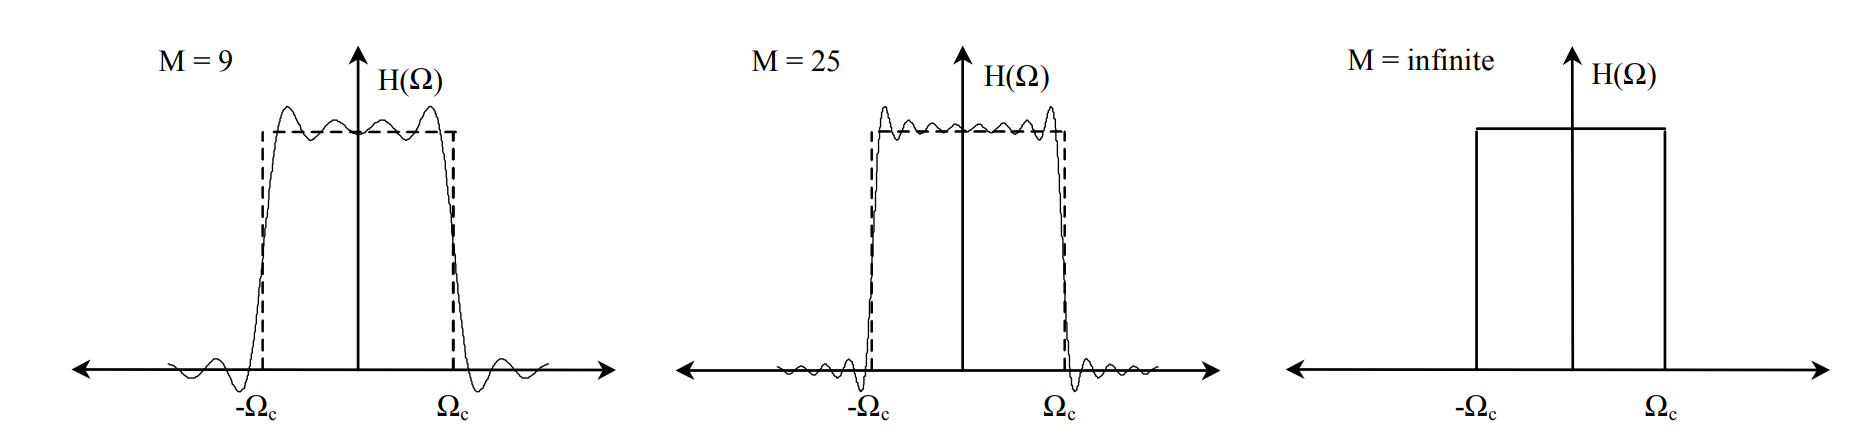
\includegraphics[width=\textwidth]{finite_trunc_ideal_filter.png}
    \caption{有限截断产生吉布斯现象}
\end{figure}

为消除这些振铃,需要对频谱使用一些函数进行二次加工,这些函数称作\emph{窗函数}。窗函数能较好改变频谱特性,与理想滤波器一起构成了实际 FIR
滤波器。以海明窗(Hamming)为例:它时域上形状是钟形曲线,而频域上则对主瓣以外成分有强烈衰减。具有这种特性的窗函数作用于理想滤波器以后,会
大幅度削减截断频率处的波纹。常见窗函数表达式与设计方法可以参考\cite[\href{https://ccrma.stanford.edu/~jos}{JULIUS O. SMITH III}]
{smith2007introduction}提供的内容。
$$\textrm{海明窗}\quad w[n]=0.54-0.46\cos(\frac{2\pi n}{N-1})$$
\begin{figure}[htbp]
    \centering\label{hamming_resp}
    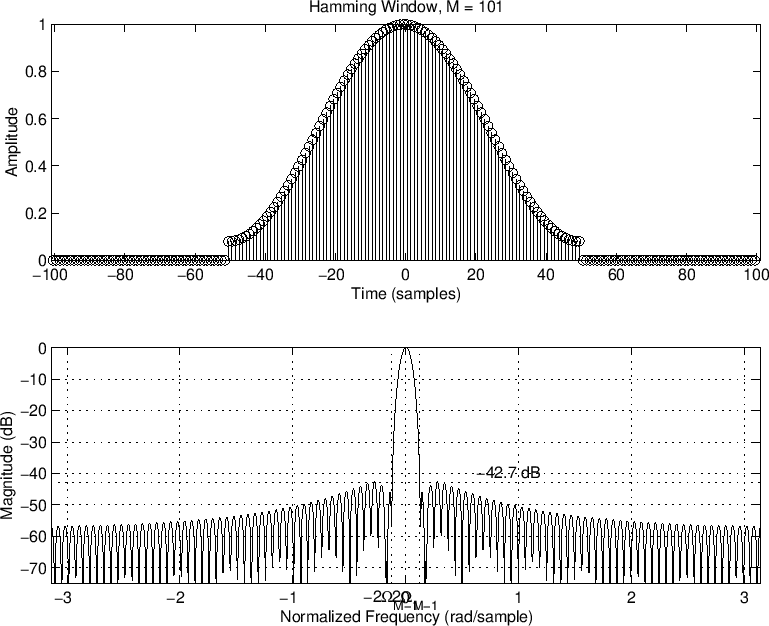
\includegraphics[width=0.8\textwidth]{hamming_resp.png}
    \caption{海明窗时域与频域形状}
\end{figure}

将窗函数叠加到理想滤波器系数,就得到最终 FIR 滤波器系数 $h[n]\leftarrow h[n]*w[n]$。图\ref{ideal_hamming_comp} 说明了加窗对滤波器性能的
影响:首先是截至频率($f_c=0.2$)处的振铃消失,此外滤波器通带与阻带的区别越发明显。
\begin{figure}[htb]
    \centering\label{ideal_hamming_comp}
    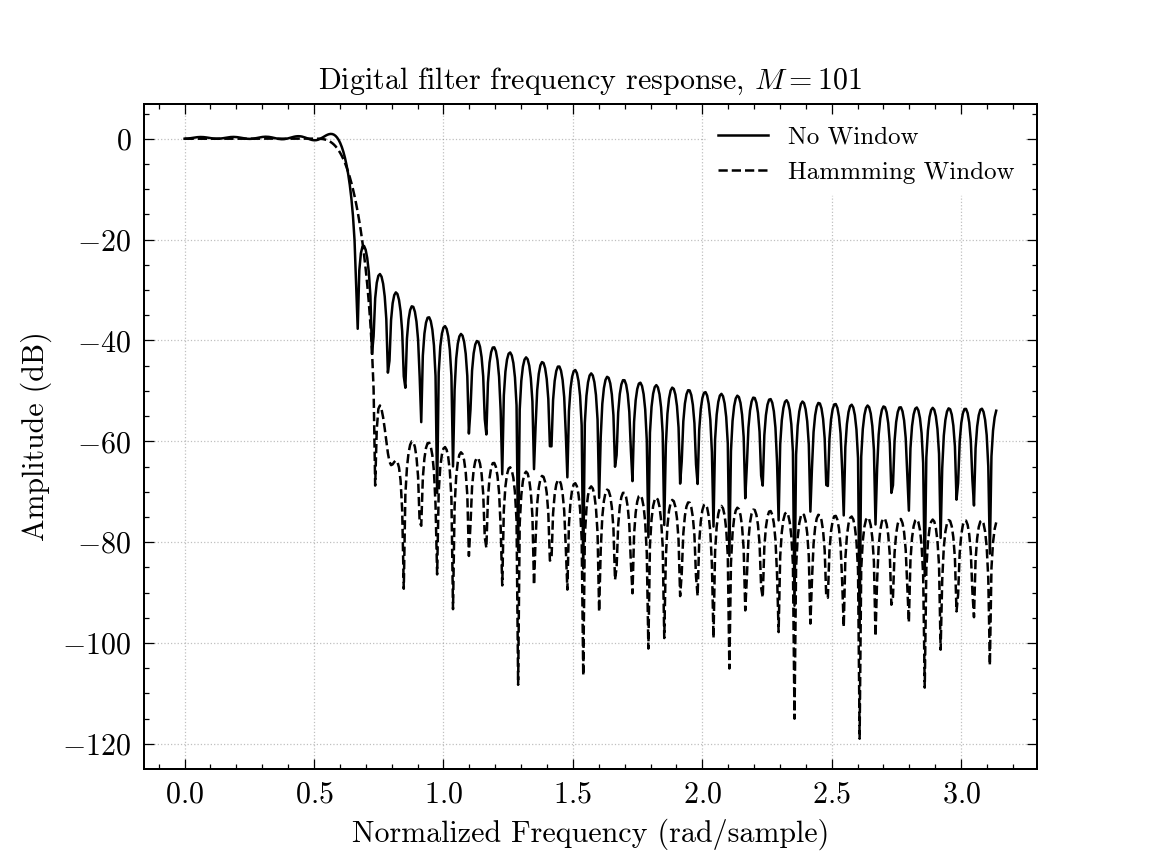
\includegraphics[width=\textwidth]{ideal_hamming_comp.png}
    \caption{理想低通滤波器幅值频幅响应}
\end{figure}
\newpage

\subsection{程序实现}
线性滤波的程序实现围绕式\ref{flt_time_domain}进行。该式表明数字线性滤波器是两项卷积之和,每项卷积有图\ref{lin_flt_impl} 表示的加乘累计
结构。这种结构易于电路与软件实现:置换卷积对应于固定位置索引与先进先出(FIFO)的队列元素的乘积和。将滤波器系数置入固定数组,然后将队列元素
依次加成就得到滤波结果。
\begin{figure}[!h]
    \centering\label{lin_flt_impl}
    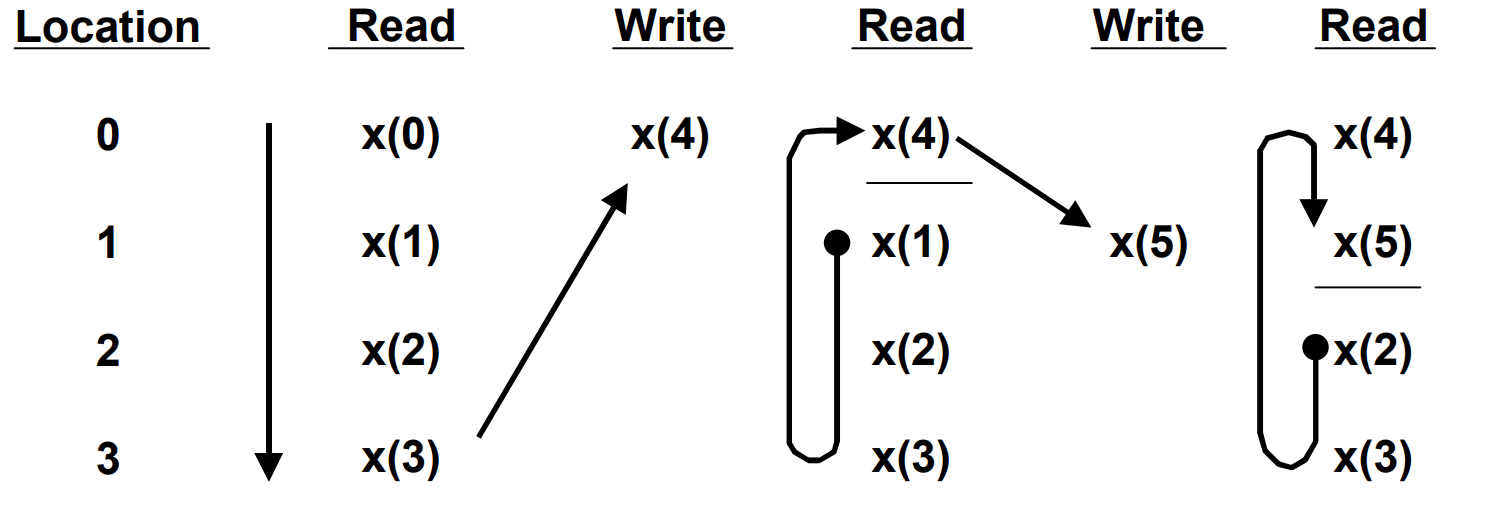
\includegraphics[width=\textwidth]{lin_flt_impl.png}
    \caption{数字滤波器的程序实现}
\end{figure}

\subsubsection{用户接口}
\textbf{Filter} 类是 ppx 实现的一般统计线性滤波器设计与使用接口,定义对应有理传递函数有如下形式:
$$
    Y(z)=\frac{b(1)+b(2) z^{-1}+\ldots+b\left(n_{b}+1\right) z^{-n_b}}{1+a(2) z^{-1}+\ldots+a\left(n_{a}+1\right) z^{-n_{a}}} X(z)
$$
这种形式能同时处理FIR与IIR型滤波器,其中 $n_a$ 是反馈滤波器阶数,$n_b$ 是前馈滤波器阶数。由归一化设定 $a(1)=1$。
该类型提供接口如下:
\begin{table}[!h]
    \centering
    \begin{tabular}{cc}
        \toprule
        \emph{构造方法} &                        \\
        \midrule
        constructor & 滤波器类型:低通(默认值)/高通/带通/带阻 \\
        \midrule
        \emph{成员方法} &                        \\
        \midrule
        coff\_a     & 返回反馈滤波器系数              \\
        coff\_b     & 返回前馈滤波器系数              \\
        reset       & 重置滤波器状态                \\
        operator()  & 滤波操作                   \\
        \bottomrule
    \end{tabular}
\end{table}

\subsubsection{使用示例}
使用有理传递函数 $H(z)=\frac{1}{1-0.9z^{-1}}$ 对数据进行滤波。创建由正弦谐波与白噪声组合的输入数据:

\begin{lstlisting}[language=C++]
    #include <iostream>
    
    int main() {
        std::cout << "Hello, World!" << std::endl;
        return 0;
    } 
\end{lstlisting}
\newpage
\bibliographystyle{unsrt}
\bibliography{references}